% -*-latex-*-

%% This is an example first chapter.  You should put chapter/appendix that you
%% write into a separate file, and add a line \include{yourfilename} to
%% main.tex, where `yourfilename.tex' is the name of the chapter/appendix file.
%% You can process specific files by typing their names in at the
%% \files=
%% prompt when you run the file main.tex through LaTeX.

\chapter{Introduction}
\label{Introduction}


\section{High Energy Electron Scattering}
%Rise the question! The history of QCD, traditional nuclear physics

%In 1911, Ernest Rutherford formulated his model of atom by interpreting the data of his gold foil experiment: a dense
%charged nucleus containing most of atom's mass, was surrounded by an electron cloud.

%As time went on, it was found that nucleus itself is composed of more fundamental particles which are called nucleons.
%Nucleons are the building blocks of the traditional nuclear physics. The properties of free nucleons have been studied
%quite well.
%However, in nuclei, nucleons are in bound state and their properties will be affected by the nuclear medium.
%The question of how nuclear medium will change the properties of nucleons is of great interest and yet still unsolved.
%

Quantum chromodynamics, or QCD, is the theory that describes the action of the strong force that binds quarks together to form baryons and
mesons, and results in the complicated the force that binds atomic nucleon together. QCD is successful in the very high energy (short distance) domain
i.e. weak coupling regime, in which a perturbative approach is valid. On the other hand, traditional nuclear physics theories work well in the
low energy (long range) domain. However, in the medium-high energy region around 1 GeV, techniques of perturbative QCD are invalid and both
QCD and traditional nuclear physics have major difficulties. A fundamental question in nuclear physics is: How can one place the low energy theories
and high energy theory (QCD) into a more general frame, on the basis of a fundamental theory? How does one connect the descriptions of long range
and short range phenomena? To answer the questions, it is essential to understand the phenomena in the medium-high energy region. Building a
bridge between nuclear physics and particle physics is an important step in the progress of physics.

The building blocks of traditional nuclear physics are nucleons. To study the structure and properties of nuclei, we
need to understand the hehaviors of nucleons in nuclei. The properties of free nucleons have been studied very well.
But nucleons in nuclei are in bound states, and their properties will be affected by nuclear medium.
How medium modifications of the nucleon form factor inside the nuclei is an essential question in nuclear physics.

To investigate the properties of nucleons in nuclear medium, the electron is used as a probe, which has several 
advantages over hadrons. The interaction between the electron and nuclei is much weaker than strong interaction.
So the electron will not disturb the nucleus as much as a hadron probe, so the physics is easier to study compare
with the more complicated nucleus-probe system.
Besides, the electron probe interact with the electro-magnetic interaction, which is very well understood through
Quantum Electrodynamics (QED). So electron probe can provide us the most useful information about nucleon and nuclear
structure.

\section{Inclusive Electron Scattering Spectrum}

Figure.~\ref{fig:scattering_spectrum}  shows a cross section spectrum for a typical inclusive scattering a nuclear target.
In inclusive scattering, only the scattered electron's energy and momentum are measured by detectors.

\begin{figure}[h]
\centering
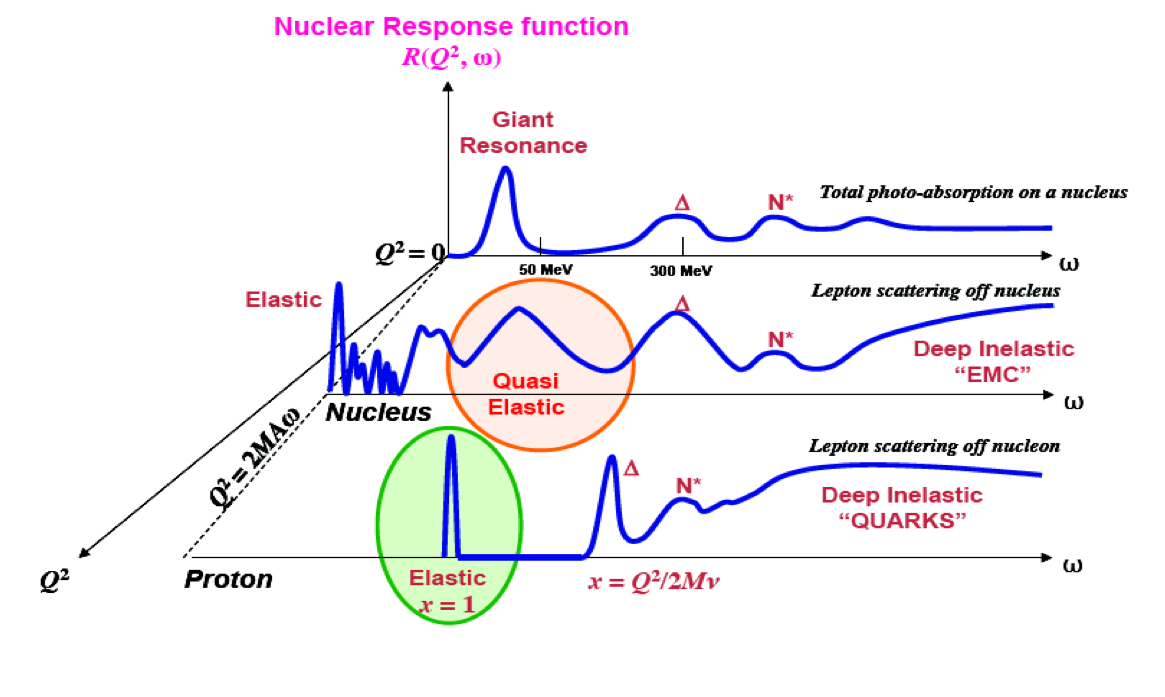
\includegraphics[width=0.8\textwidth]{figs/scattering_spectrum.png}
\caption[scattering spectrum]{Nuclear responses to electron scattering \label{fig:scattering_spectrum}}
\end{figure}

In electron inclusive scattering, as the energy loss $\omega$ increase, different nuclear response structures can
be observed.
The nuclear response structures can be classified as: elastic peak, nuclear excitation levels, giant resonance,
quasi-elastic peak, meson exchange currents (MEC), $\Delta$ peak, higher resonances, and deep inelastic scattering
(DIS).

The first structure can be seen is the elastic peak at $\omega = Q^2/2M$( $Q$ is four momentum transfer and $M$ is the
nucleus mass), the electron's energy loss equal to recoil energy of nucleus.
When the electron's energy loss is larger than the recoil energy, the nucleus will go into an excitation state.
These excitation states correspond to the excitation peaks in the spectrum.

When the energy loss is large enough the electron can knock out a single nucleon from the nucleus, this correspond to
the quasi-elastic peak in the energy loss spectrum. The quasi-elastic peak is a broad peak located above $Q^2/2M_N$ ($M_N$
is the mass of nucleon), the shift of center of the quasi-elastic peak from $Q^2/2M_N$ is due to the average
separation energy. The nucleon motion in nucleus will cause the quasi-elastic peak broadening, and the width of the peak
is characterized by Fermi momentum $k_F$ and momentum transfer $|\vec{q}|$.

If the energy loss continue increase, the knocked out nucleon will be excited into a $\Delta$ resonance state. 
%The $\Delta$ peak is much broader than quasi-elastic peak. 
After the $\Delta$ resonance, there is deep inelastic region and continuum states.

%models, longitudinal and transverse response function

\section{Quasi-elastic Electron Scattering}

In an quasi-elastic inclusive unpolarized electron nucleus scattering process, an electron with initial energy $E$ and
momentum $\vec{k}$ scattered off a rest nucleus of mass $M_N$.
The scattered electron is then measured at angle $\theta$ with scattered energy $E'$ and momentum $\vec{k'}$ by detector package.
The process happens with the exchange of a virtual photon $\gamma (\omega, \vec{q})$,
where $\omega = E - E'$, $\vec{q} = \vec{k} - \vec{k'}$ .
%The Feynman diagram of this process at lowest order of $\alpha$ and with plane wave impulse approximation is show in Figure.~\ref{fig:quasi-elastic_diagram}.

\begin{figure}[h]
\centering
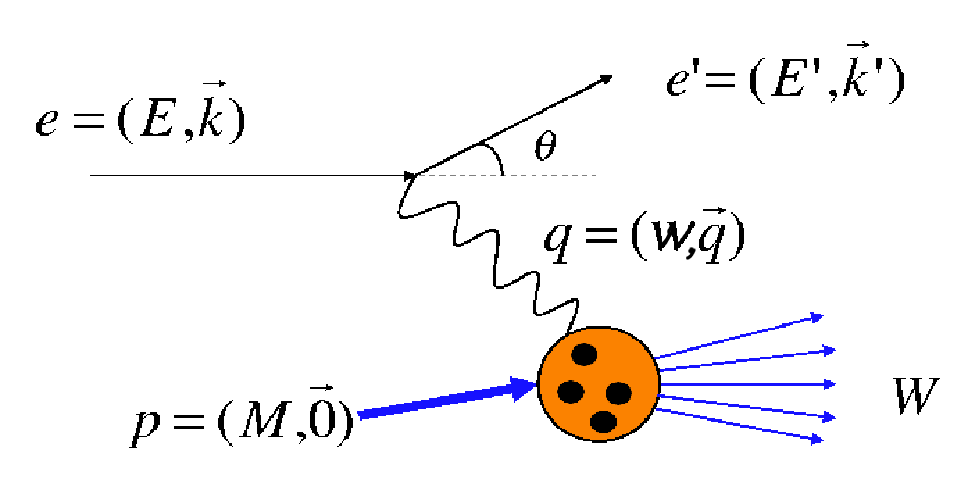
\includegraphics[width=0.8\textwidth]{figs/feynman_diagram.png}
\caption[scattering spectrum]{Quasi-Elastic electron scattering \label{fig:feynman_diagram}}
\end{figure}

With the Born approximation, the differential cross section of the inclusive unpolarized electron scattering described above can be written as:
\begin{equation}
%  \sigma \equiv \frac{d\sigma}{d\Omega d\omega} = \sigma_M [\frac{Q^ 4}{\bm{q}^4}R_L(|\bm{q},\omega|)+\frac{Q^2}{2\bm{q}^2}\frac{R_T(|\bm{q},\omega|)}{\varepsilon}]
%  \sigma \equiv \frac{d\sigma^3}{d\Omega d\omega} = \sigma_M \left[ W_2(|q|,\omega) + 2W_1(|q|,\omega)\tan^2\left(\frac{\theta}{2}\right) \right]
\frac{d\sigma^3}{d\Omega d\omega} = \sigma_M \left[ W_2(|q|,\omega) + 2W_1(|q|,\omega)\tan^2\left(\frac{\theta}{2}\right) \right]
\end{equation}


\begin{equation}
  \sigma_M=\frac{4\alpha^2 \cos^2(\theta/2)}{4E^2\sin^4(\theta/2)}
\end{equation}

is the  Mott cross-section for scattering electrons from a point-like infinitely heavy target. 
It is convenient to separate contribution of longitudinal and transverse polarized virtual photon:
%The right side of this equation can also be re-written to separate contributions of longi- tudinally and transversely polarized virtual photons to the scattering processes
\begin{equation}
\frac{d\sigma^2}{d\Omega d\omega} =  \sigma_M \left[ \frac{Q^4}{\vec{q}^4}R_L(|\vec{q},\omega|)+\frac{Q^2}{2\vec{q}^2\varepsilon}R_T(|\vec{q},\omega|) \right]
\end{equation}


where 

\begin{equation}
Q^2 = \vec{q}^2 - \omega^2
\end{equation}

gives the four momentum squared of the exchanged virtual photon;

\begin{equation}
  \varepsilon(|\vec{q}|,\omega,\theta) =\left[1+\frac{2\vec{q}^2}{Q^2}\tan^2\frac{\theta}{2}\right]^{-1}
\end{equation}

is virtual photon polarization.
This is the Rosenbluth formula.
%a brief derivation is provided in Appendix A for reader's convenience.

The relation of $R_L$ and $R_T$ with $W_1$ and $W_2$ is given by: 
\begin{equation}
R_T(|\vec{q}|)=2W_1(|\vec{q}|)
\end{equation}

and

\begin{equation}
\frac{Q^2}{|\vec{q}|^2}R_L(|\vec{q}|)=W_2(|\vec{q}|) - \frac{Q^2}{|\vec{q}|^2}W_1(|\vec{q}|)
\end{equation}

$R_L$ is the longitudinal response function, $R_T$ is the transverse response function of nucleus.
$R_L$ measures the nuclear charge and $R_T$ measures the magnetic component of the electromagnetic current of the
nucleus. Experimentally the $R_L$ and $R_T$ can be extracted by measuring cross section at a given $(Q^2,\omega)$ at
two or more angles. Then a plot of $\varepsilon \frac{d\sigma^2}{d\Omega d\omega}/\sigma_M$ vesus $\varepsilon$ should 
fall on a straight line. The slope of this line is $(Q^4/\vec{q}^4)R_L$, the intercept is $(Q^2/2\vec{q}^2)R_T$.

\section{Coulomb Sum Rule}

The Coulomb Sum is defined as the integration of longitudinal response function $R_L(|\vec{q}|,\omega)$ divided by 
nucleon charge form factor over the full range of energy loss $\omega$ at a constant three momentum transfer $q \equiv |\vec{q}|$:

\begin{equation}
C_{in}(q) = \int_{\omega_{el}^{+}}^{q} \frac{R_L(|q|,\omega)}{F_1^2(Q^2)} d\omega = Z + \Delta C
\end{equation}

where $F_1^2(Q^2)$ is nucleon charge form factor. $\omega_{el} = Q^2/2M$, $\omega_{el}^{+}$ mean just above the elastic peak. 
Z is the charge number of the target nucleus, and $\Delta C$ is the two-nucleon correlation function.

The relativistic effects and the neutron contributions can be considered as corrections:
\begin{equation}
\tilde{G}^2_E = |\tilde{G}^p_E(Q^2)|^2 + (N/Z) |\tilde{G}^n_E(Q^2)|^2
\end{equation}

\begin{equation}
\tilde{G}^{p(n)}_E(Q^2) = G^{p(n)}_E(Q^2) \sqrt{\frac{1+Q^2/4m^2_N}{1+Q^2/2m^2_N}}
\end{equation}

where $m_N$ is the nucleon mass, N is the neutron number of the nucleus, and $G^{p(n)}_E$ is the proton (neutron)
charge form factor.

At high momentum transfer, another form of Coulomb sum is defined:

\begin{equation}
S_L(Q^2) = \int_{\omega_{el}^{+}}^{\omega_{max}} \frac{R_L(Q^2,\omega)}{|\tilde{G}_E(Q^2)|^2}
\end{equation}

where $\omega_{max}$ is the maximum value of the energy defined by the virtual mass of the exchanged photon:
$\omega < |\vec{q}|$. Here we define $S_L$ as a function of $Q^2$ instead of $|\vec{q}|$, because $Q^2$
a Lorentz invariant.Since it is defined only in the physical region
($Q^2>0$), the problem of strength from outside the physically accessible region is
also avoided.

$S_L$ is predicted to be unity, when $q \gg k_f$, $k_f$ is the fermi momentum of the nucleus.
%However, modifications in the electromagnetic properties of the free nucleons by
%the nuclear medium (EMC effect) and the presence of short range correlations can change
%this result. It is generally accepted that $S_L$ shouldn't quench more than a few percent
%at $q = 2k_f$ and reach 1 at higher $q$ values. The validity of reaching unity at high $q$
%is model independent. 
Here are a few corrections to Coulomb Sum Rule:

\begin{itemize}
\item Finite size effect:  
The finite size effect is due to center-of-mass motion. The total Coulomb Sum is not affected by the center-of-mass
correlations,but in actual calculation of CSR one is faced with the difficulty of subtracting spurious center-of-mass 
effect from the nuclear charge form factor.
This effect become smaller with increasing mass number, as shown in Figure.~\ref{fig:finite_size_data}. And this correction is important for
small $q$. 

\begin{figure}[h]
\centering
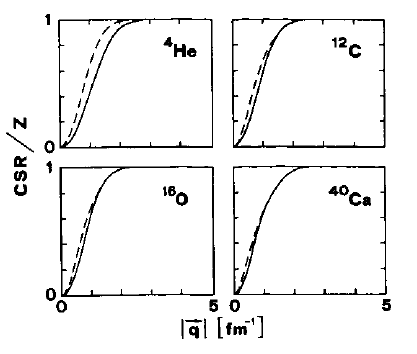
\includegraphics[width=0.7\textwidth]{figs/finite_size_data.png}
\caption[finite size data]{CSR divided by the proton number, as a function of the three-momentum transfer, in the
harmonic oscillator model, without(broken curve) and with(full curve) center-of-mass corrections. Figure from
\cite{Orlandini1991}.  \label{fig:finite_size_data}}
\end{figure}


\item Pauli blocking: The nucleons are fermions, and the Pauli exclusion principle requires that two or more nucleons
cannot occupy the same quantum state within the same quantum system. 
The Pauli blocking is more important at small $|\vec{q}|$ and negligible at large $|\vec{q}|$. The comparison between
with and without Pauli correlations is calculated by Lightbody using harmonic oscillator model for $^{12}C$ is shown
in Figure.\ref{fig:pauli_blocking_compare}.

\begin{figure}[h]
\centering
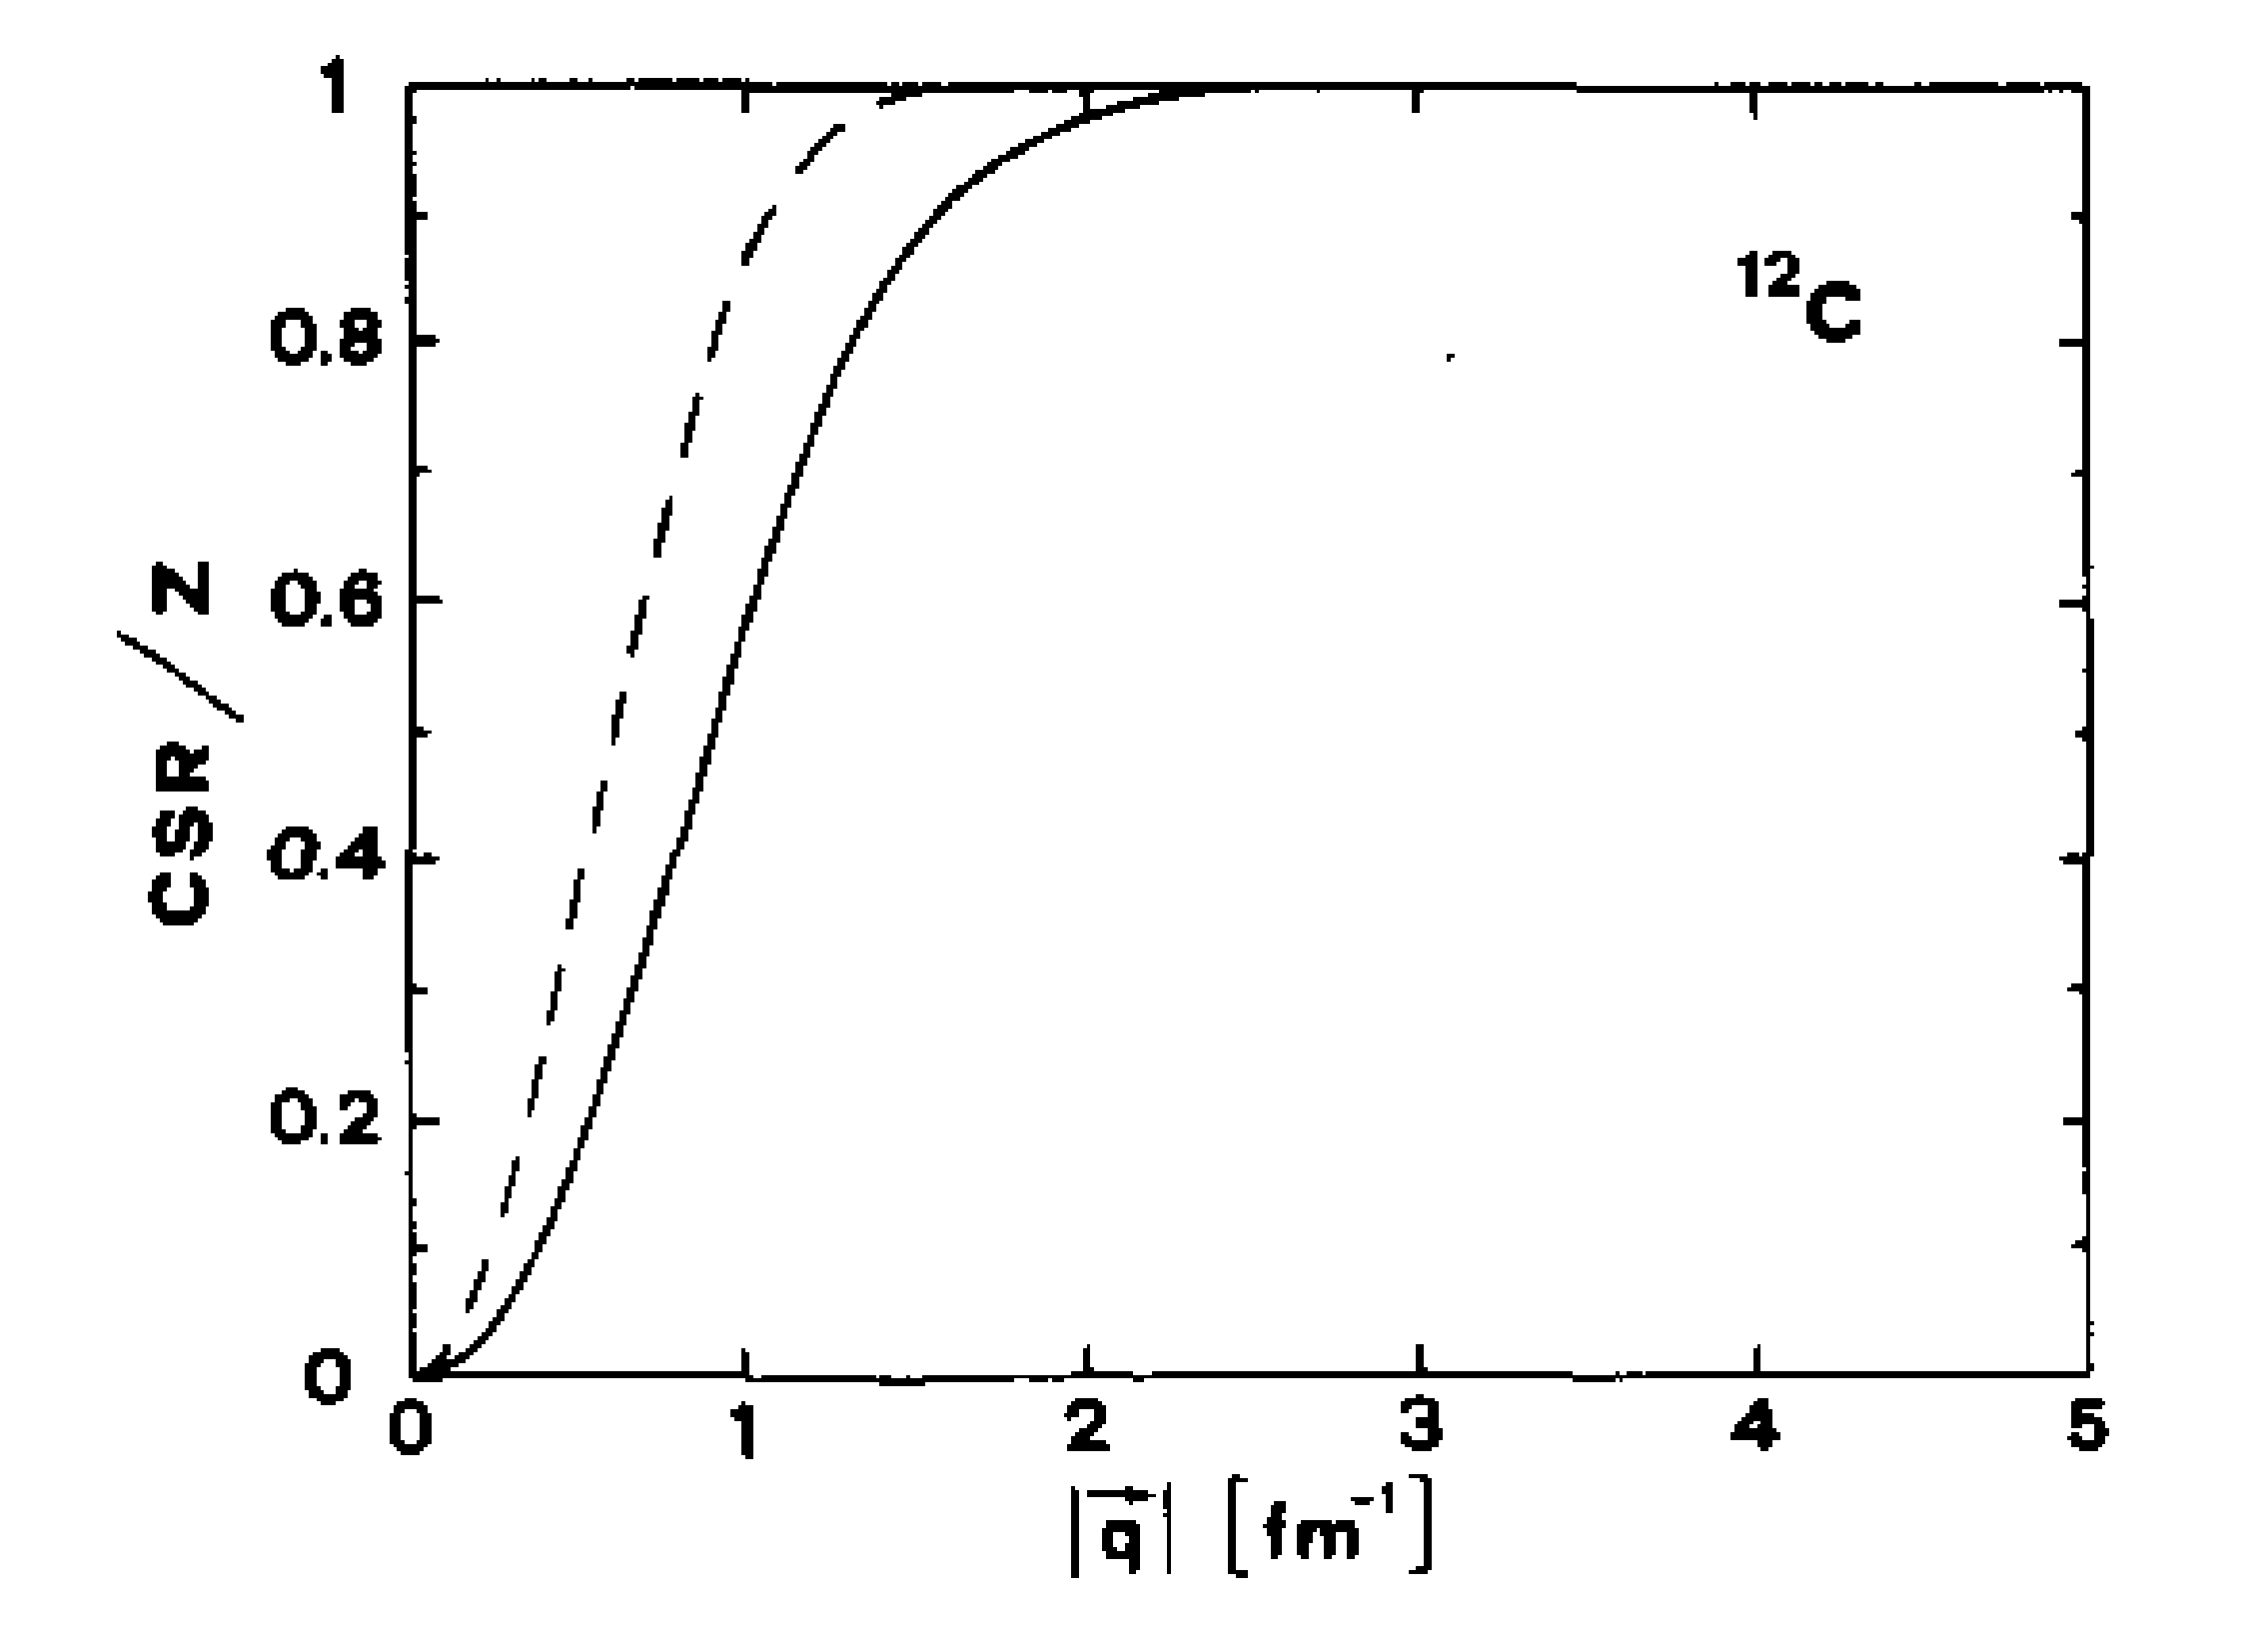
\includegraphics[width=0.7\textwidth]{figs/pauli_blocking_compare.png}
\caption[pauli blocking compare]{CSR divided by the proton number, as a function of the three momentum transfer,
without(broken curve) and with(full curve) Pauli correlations. Figure from
\cite{Orlandini1991}.  \label{fig:pauli_blocking_compare}}
\end{figure}

\item Long range correlations:
In the region of low momentum transfer, the interaction between nucleons have a long range nature and are responsible
for the giant resonances. The long-range correlation has been studied based on the random phase approximation (RPA).
The long range correlations are effective at low $q$ and vanish at high $q$.
The quenching effect on the CSR produced by the RPA is shown in Figure\ref{fig:long_range_data}:

\begin{figure}[h]
\centering
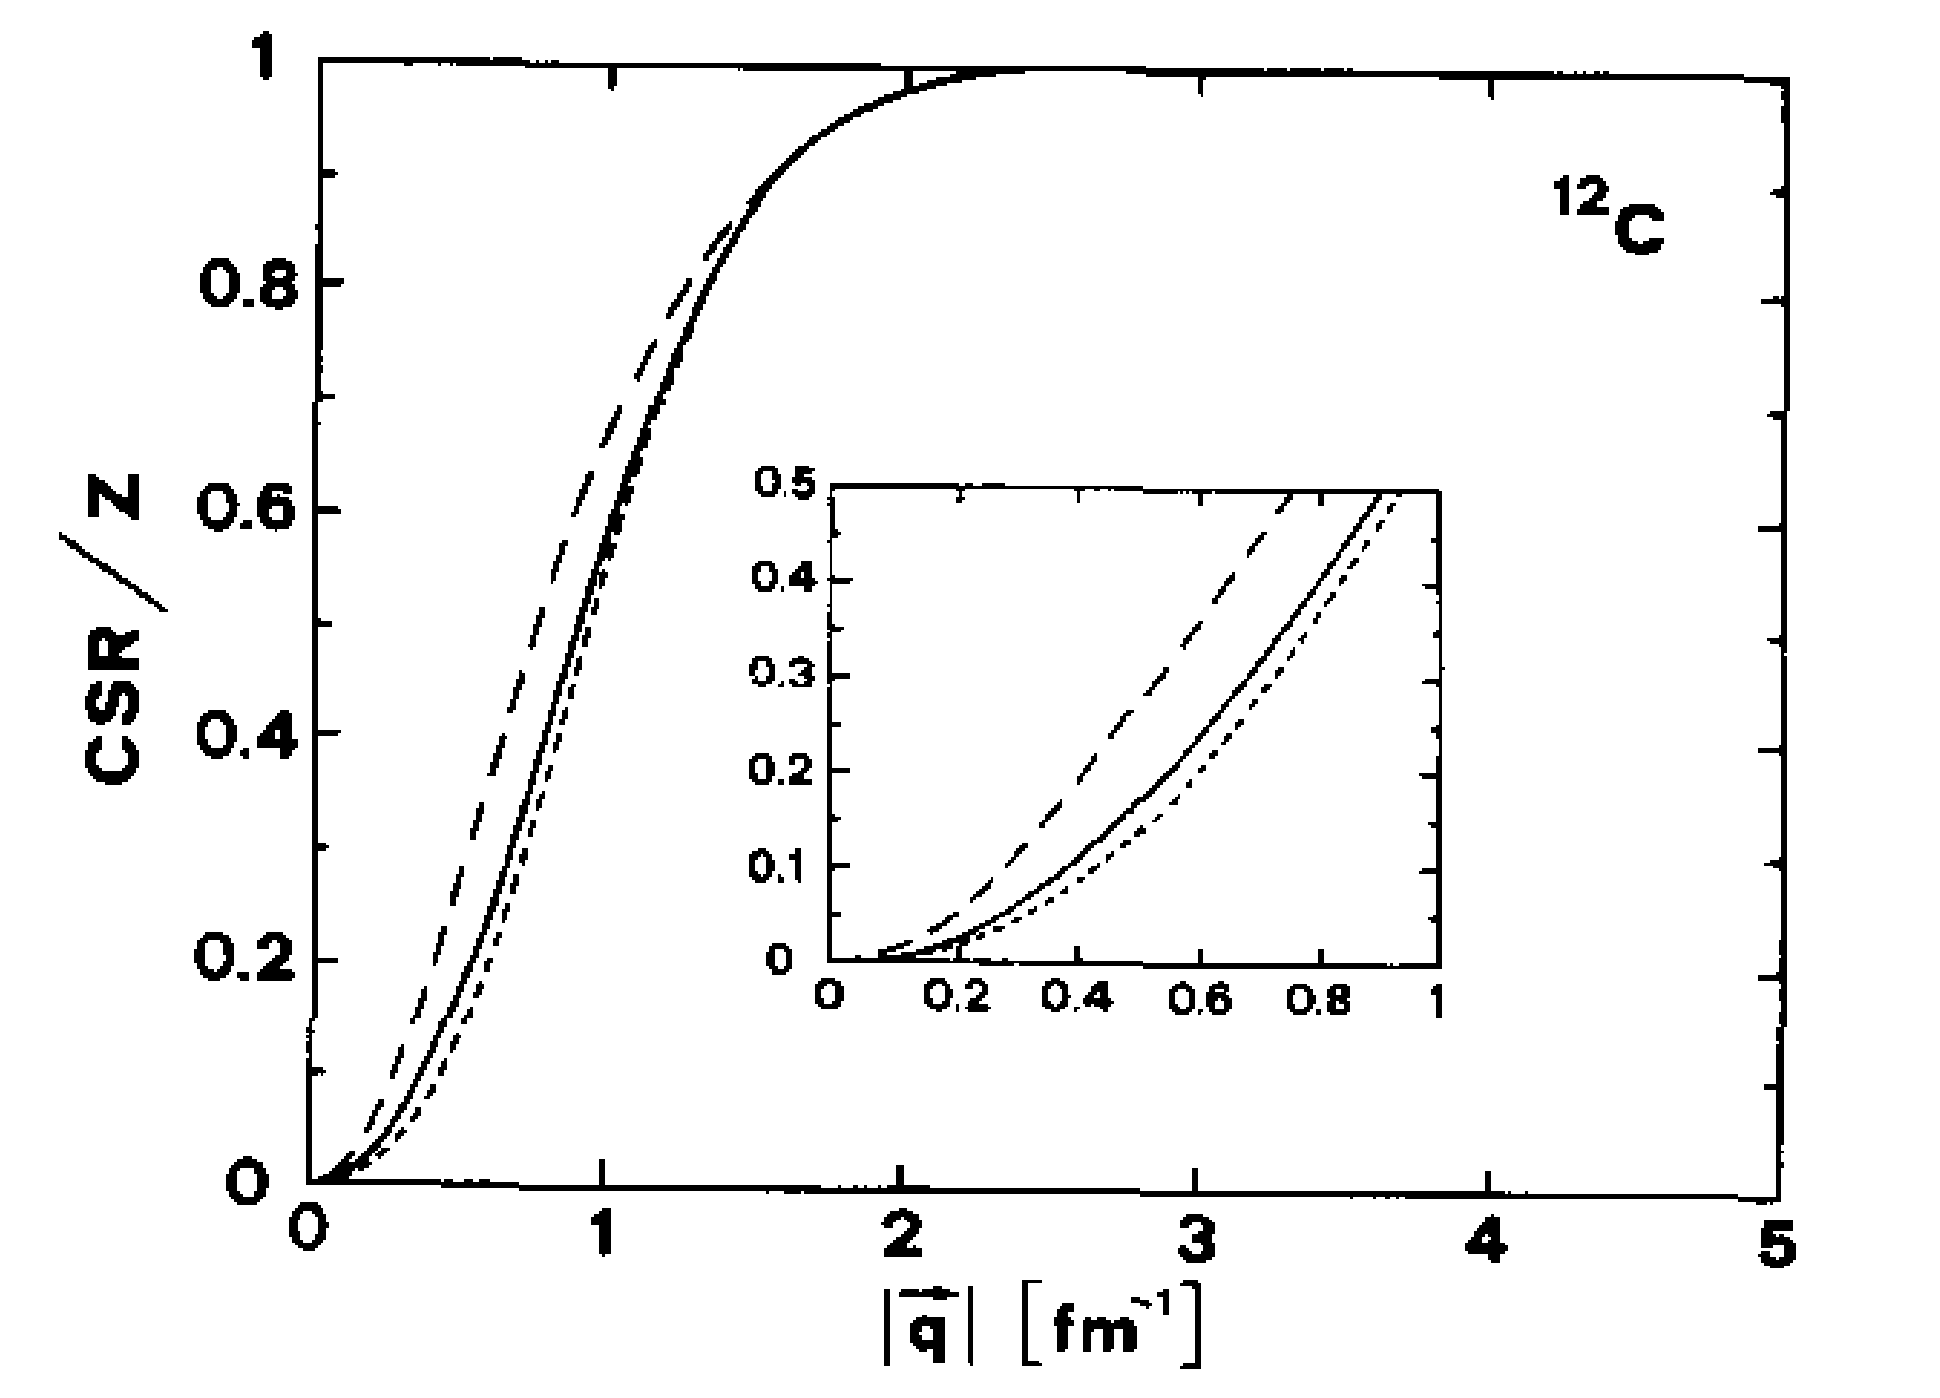
\includegraphics[width=0.7\textwidth]{figs/long_range_data.png}
\caption[long range data]{CSR divided by the proton number, as a function of the three momentum transfer in the 
harmonic oscillator model wihtout (long broken curve) and with(full curve) center-of-mass correlations.
The short broken curve represents the result including RPA correlations.
 Figure from \cite{Orlandini1991}.
\label{fig:long_range_data}}
\end{figure}

\item Short range correlations:
In the deep inelastic (DIS) region, the virtual photon explores the medium and short inter-nucleon distances \cite{Orlandini1991}.
So the longitudinal structure function is sensitive to the short range proton-proton correlations, and these can affect
the CSR to be quenched. Short-range correlations are obtained for example by modifying the
short-range behaviour of the relative proton-proton wavefunction through a Jastrow-type correlation:

\begin{equation}
g(r) = 1 - e^{\gamma \alpha^2 r^2/4}
\end{equation}

The effect of short range correlation for $^{12}$C is shown in Figure\ref{fig:short_range_data}:

\begin{figure}[h]
\centering
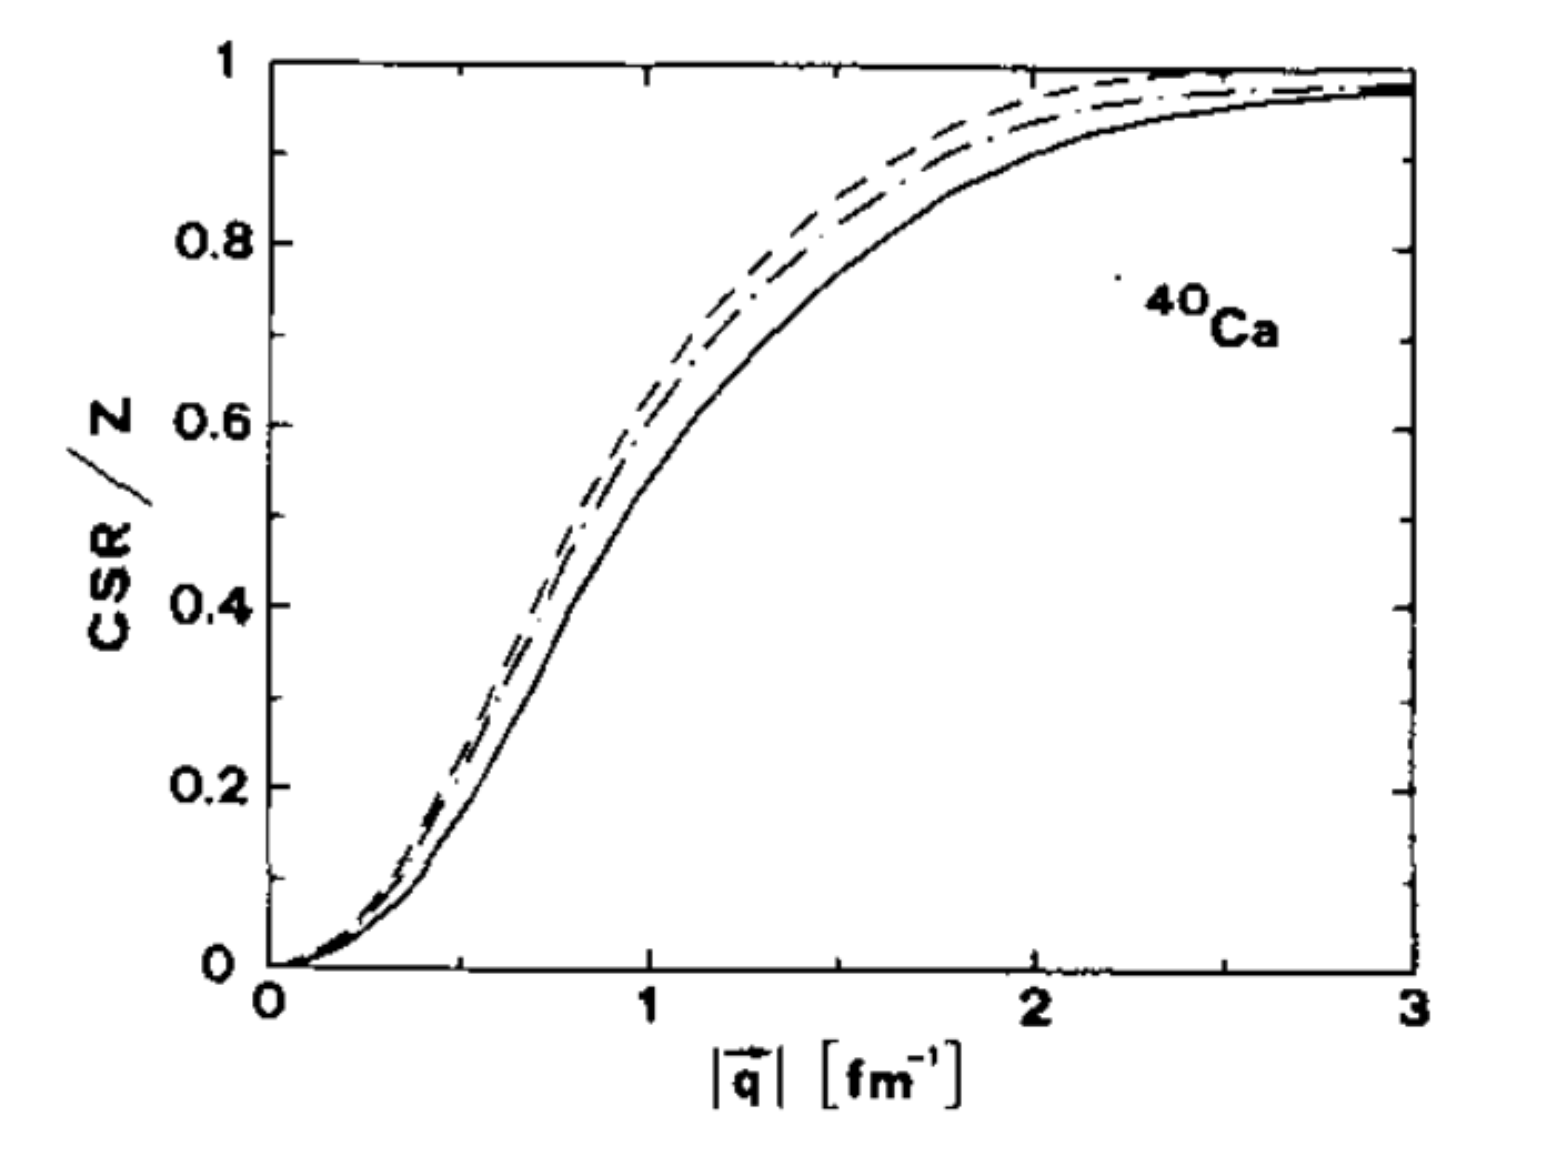
\includegraphics[width=0.7\textwidth]{figs/short_range_data.png}
\caption[short range data]{CSR divided by the proton number, as a function of the three momentum transfer in the 
harmonic oscillator model (broken curve, $\alpha_0$ = 0.51 fm$^{-1}$) and with short-range correlations included
(chain curve, $\gamma$ = 56.1; full curve: $\gamma$ = 24.9).
 Figure from \cite{Orlandini1991}.
\label{fig:short_range_data}}
\end{figure}

\end{itemize}

\section{Existing Data}
In the past thirty years, a large experimental program has been carried out at the Bates, Saclay and SLAC
aimed at the extraction of $R_L$ and $R_T$ for a variety of nuclei \cite{Meziani2001}.
The Bates and Saclay data have the resenbluth separation only performed up to $q$ = 550 MeV/c due to the maximum beam
energy limiation (~800 MeV). At SLAC only a measurement at $q$ = 1140 MeV/c was performed due to the minimum beam energy
available (~900 MeV). The large uncertainty on the SLAC data point makes it inconclusive. So experiment E05-110 at
Jefferson Lab can test Coulomb Sum Rule in the region not measured before with significantly improved precision.

The longitudinal and transverse response functions extracted with Rosenbluth separation are available for
$^2$H, $^3$H, $^3$He, $^4$He, $^{12}$C, $^{40}$Ca, $^{48}$Ca, $^{56}$Fe, $^{238}$U in the range 200 MeV/c $\leq q \leq$
600 MeV.

The experimental transverse response functions are generally in reasonable agreement with the simple model predictions.
In the kinematic region where the contributions from processes such as elastic scattering, nuclear
excitation and giant resonance are small, the agreement between theories and experiments is good.
In the region where the contributions from the other processes, such as meson exchange current (MEC) and $\Delta$ excitation are important,
the situation becomes complicated. By taking into account these contributions, theorists can still reproduce the transverse response function well.

\begin{figure}[h]
\centering
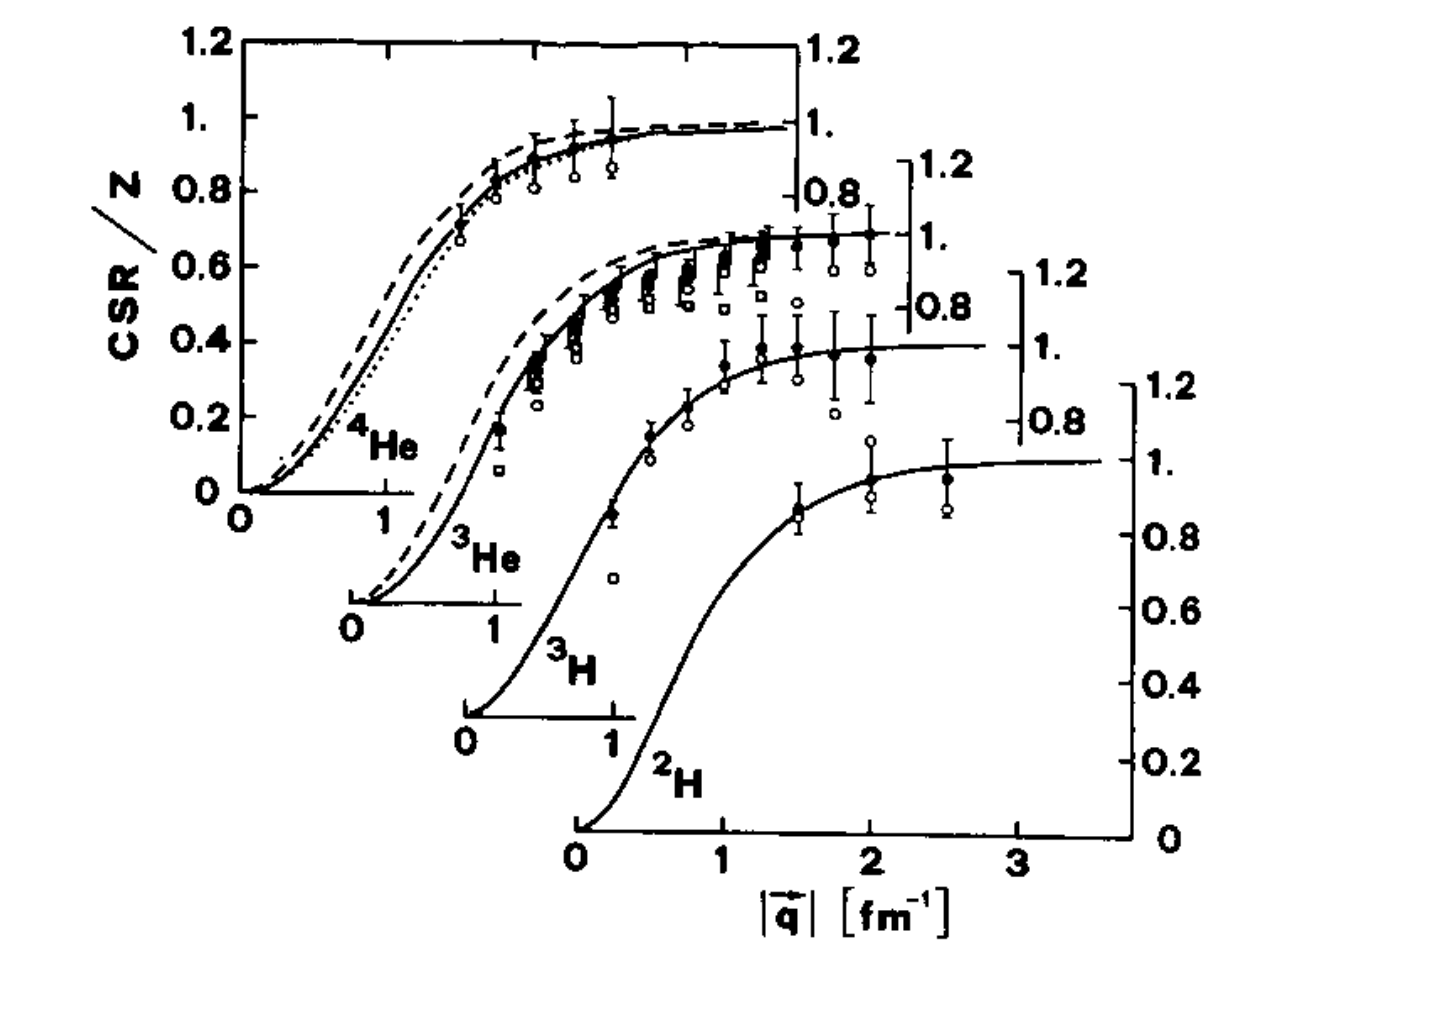
\includegraphics[width=0.7\textwidth]{figs/csr_data.png}
\caption[csr data]{The CSR divided by the proton number as a function of three momentum transfer
for light weight nuclei. Continuous curves: results from Schiavilla \cite{Schiavilla1987} ; dotted curve:
correlated model. The empty points represent the experimental values, while the filled points
are the tail corrected results. Both Saclay (circles) and Bates (squares) data are shown for $^3$He.
 Figure reproduced from \cite{Orlandini1991}.
\label{fig:csr_data}}
\end{figure}

\begin{figure}[h]
\centering
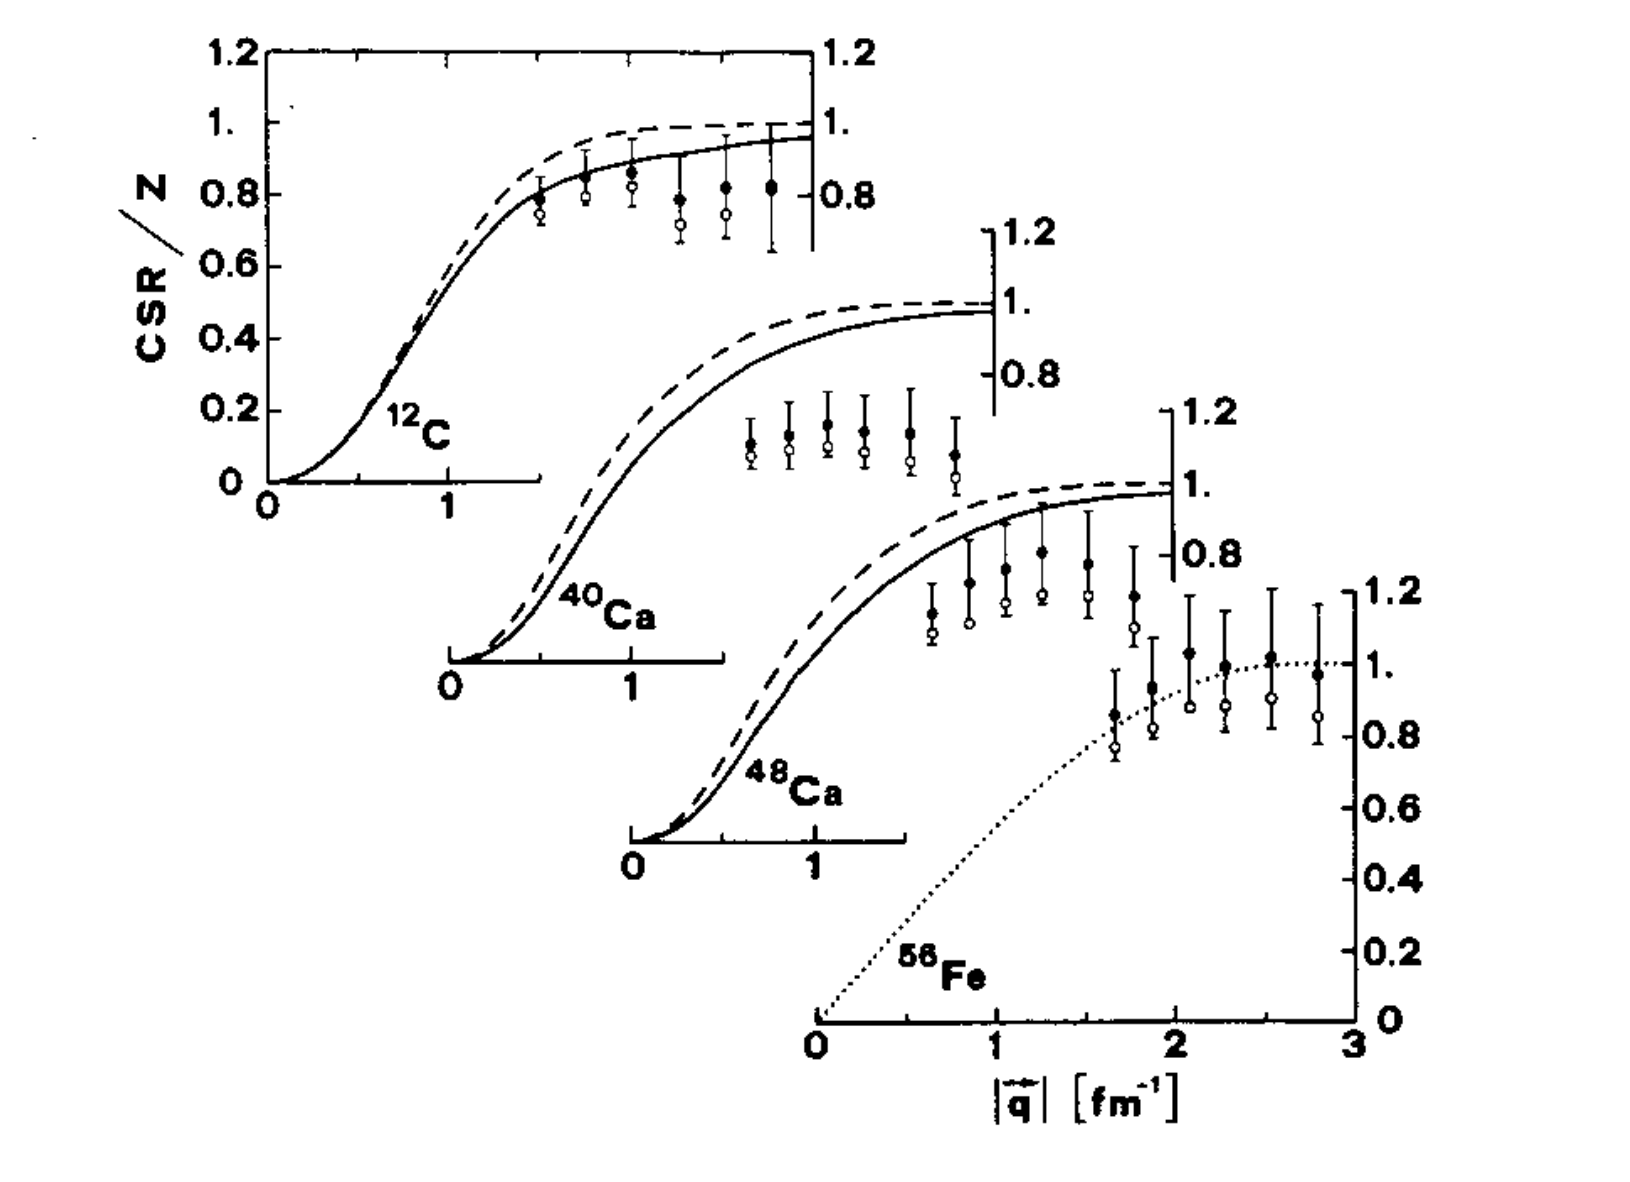
\includegraphics[width=0.7\textwidth]{figs/csr_data_2.png}
\caption[csr data2]{The CSR divided by the proton number as a function of three momentum transfer
for medium weight nuclei. Broken curves: harmonic oscillator; Continuous curves: correlated
model; Dotted curve: Fermi gas model, $k_f$ = 1.32 fm$^{-1}$. The empty points represent the
experimental values from Saclay, while the filled points are the tail corrected results.
 Figure reproduced from \cite{Orlandini1991}.
\label{fig:csr_data2}}
\end{figure}

For the longitudinal response function, the agreement between calculation and experiment is reasonably good
for light nuclei, such as $^2$H, $^3$H, $^3$He. For medium-weight to heavy nuclei(Figure \ref{fig:R_LT_q_410}
,\ref{fig:R_LT_q_550}),
there is an obvious
quenching for the experimental longitudinal response function. The quenching of $R_L$ has a clear
dependence on the nuclear mass number $N$. Besides, the quenching has a dependence on the momentum transfer:
the discrepancy between experimental $R_L$ and simple Fermi gas model calculation becomes smaller when $q$
increases. This feature can be explained by the Pauli correlation, which decrease quickly when $q$ increases.


\begin{figure}
\begin{subfigure}{.7\textwidth}
\centering
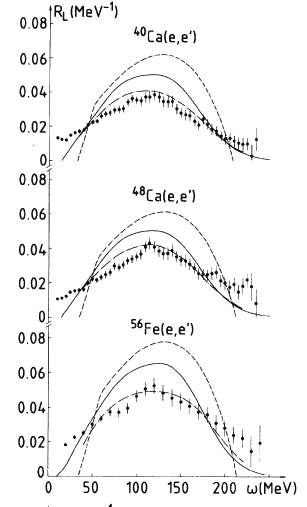
\includegraphics[width=.8\linewidth]{figs/R_L_q_410.png}
\label{fig:R_L_q_410}
\end{subfigure}%
\begin{subfigure}{.5\textwidth}
\centering
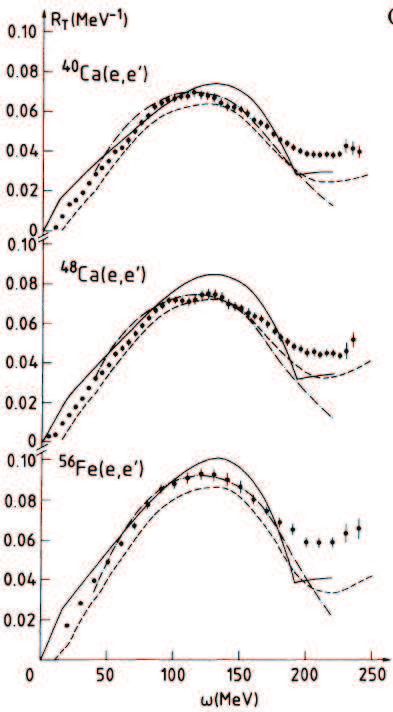
\includegraphics[width=.8\linewidth]{figs/R_T_q_410.png}
\label{fig:R_T_q_410}
\end{subfigure}
\caption[R LT q 410]{
(a) $R_L$ and (b) $R_T$ of $^{40}$Ca, $^{48}$Ca, and $^{56}$Fe at $|\vec{q}|$ = 410 MeV/c.
(a) The dashed line is a Fermi-gas caculation by Van Orden; the solid
line, a shell model calculation by Laget; and the dot deshed line a calculation
by Do Dang. (b) The dashed line is the total contribution from calculation
by Laget. The dot-dashed line is the Do Dang and Va Giai calculation
containing only the quasi-elastic process. The solid line is the random-
phase approximation (RPA) calculation with 1p-1h and 2p-2h excitations
by Alberico, Ericson, and Molinari.
\label{fig:R_LT_q_410}}
\end{figure}


\begin{figure}
\begin{subfigure}{.7\textwidth}
\centering
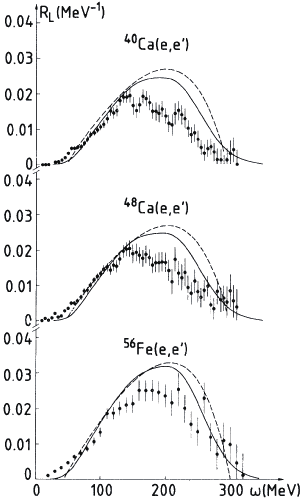
\includegraphics[width=.8\linewidth]{figs/R_L_q_550.png}
\label{fig:R_L_q_550}
\end{subfigure}%
\begin{subfigure}{.5\textwidth}
\centering
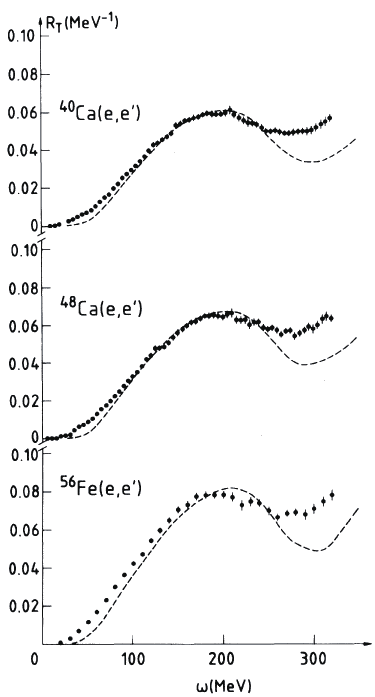
\includegraphics[width=.8\linewidth]{figs/R_T_q_550.png}
\label{fig:R_T_q_550}
\end{subfigure}
\caption[R LT q 550]{
(a) $R_L$ and (b) $R_T$ of $^{40}$Ca, $^{48}$Ca, and $^{56}$Fe at $|\vec{q}|$ = 550 MeV/c.
Description of curves are same as in Figure \ref{fig:R_LT_q_410}
\label{fig:R_LT_q_550}}
\end{figure}

The Coulomb Sum Rule is extracted from the data mentioned above with three momentum transfer in the range
200 MeV/c $\leq q \leq$ 550 MeV/c, by integrating $R_L$ over the experimental measured region of energy loss
$\omega$. As shown in Figure\ref{fig:S_L_data}, the light nuclei ($^{3}$He) reach unity at high $q$ quickly.
There is a clear sign of quenching from theoretical calculation up to 40\% for medium ($^{56}$Fe, $^{40}$Ca and
$^{48}$Ca) and heavy nuclei ($^{208}$Pb).

\begin{figure}[h]
\centering
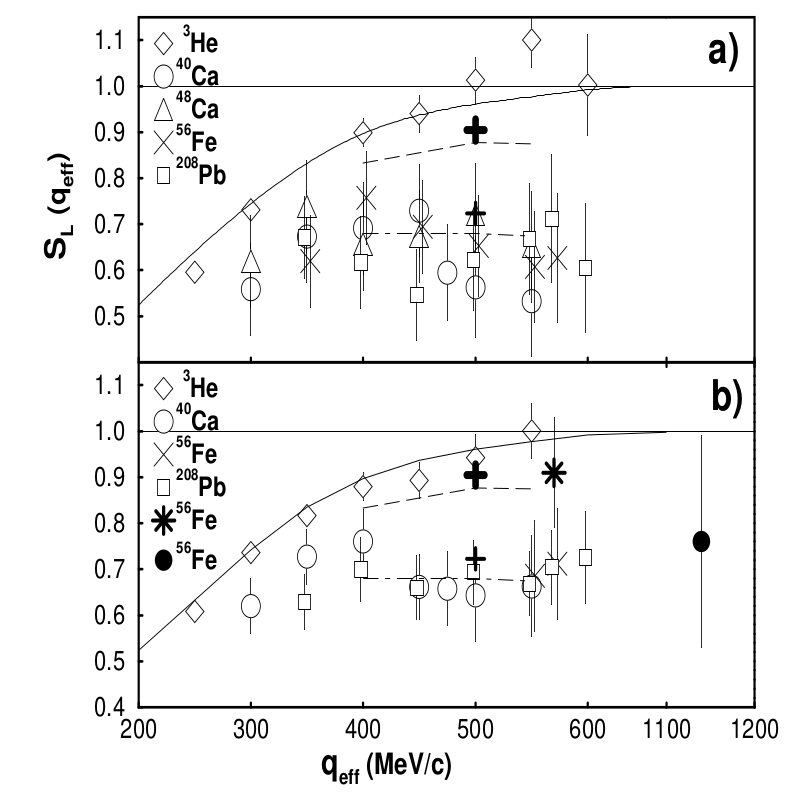
\includegraphics[width=0.7\textwidth]{figs/S_L_data.png}
\caption[S L data]{
5. Longitudinal (a) and transverse (b) response functions of $^{208}$Pb at
$q_{eff}$ = 550 MeV/c extracted in the EMA. Saclay data only (filled circles), combined with $^{197}$Au \SI{15}{\degree} SLAC data (triangles
up), combined with Bates $^{238}$U \SI{60}{\degree}
data (triangles down); previous Saclay results with Coulomb corrections [19]:
thin solid lines. c) Longitudinal response function at $q_{eff}$ = 500 MeV/c (same
experimental symbols). Nuclear matter calculations: dashed line, Hartree
Fock calculations including short range correlations and final state interactions with free nucleon form factors
(solid line), with modified nucleon
form factors (dotted-dashed line).
Figure reproduced from \cite{Meziani2001}.
\label{fig:S_L_data}}
\end{figure}


A later analysis on Saclay and SLAC data by Jourdan\cite{Jourdan1995} suggested that no quenching
exists by using the distorted wave Born approximation with the Coulomb corrections.
However, reanalysis of Saclay Data by Morgenstern and Meziani\cite{Meziani2001} with the effective
momentum approximation showed that quenching still exists. The comparison between
Morgenstern and Meziani's analysis and Jourdan's work is presented in Table \ref{tab:calc_compare}.
Two differences are identified: (a) the Coulomb corrections and (b) the use of the total error in
the Saclay data but only the statistical error in the SLAC data by Jourdan.

\begin{table}[tb!]
\begin{tabular}{ccccc}
\hline
Analysis & \begin{tabular}[c]{@{}c@{}}Saclay\\ Uncertainty\end{tabular} & \begin{tabular}[c]{@{}c@{}}SLAC\\
Uncertainty\end{tabular} & Coulomb Correction & $S_L$         \\ \hline
Jourdan  & total                                                        & statistical
& No                 & 0.86$\pm$0.12 \\
         & total                                                        & statistical
         & Yes                & 0.91$\pm$0.12 \\ \hline
         M\&M     & total                                                        & (*)
         & No                 & 0.72$\pm$0.23 \\
                  & total                                                        & (*)
                  & Yes                & 0.63$\pm$0.20 \\
                           & total                                                        & total
                           & No                 & 0.82$\pm$0.12 \\
& total                                                        & total
& Yes                & 0.73$\pm$0.12 \\ \hline
\end{tabular}
\label{tab:calc_compare}
\end{table}


\section{Theoretical Models}
Since the 1980s, great efforts have been made to resove the $R_L$ quenching problem (or the missing charge problem).
The traditional non-relativistic models cannot explain the problem.

Some models including relativistic corrections, final state interactions, and two-body and many body correlations.
These effects are important but not large enough to explain all the quenching of $R_L$ if the predicted $R_T$ is 
to remain in agreement with the experiment data.

In order to explain this puzzle , several more exotic explanations have been raised:

\begin{itemize}
\item Inadequate Coulomb correction:
The idea of the Rosenbluth separation of the longitudinal and transverse re-
sponse functions is based on the Plane Wave Born Approximation (PWBA)
and one photon exchange. This approximation is not valid for medium and heavy nuclei 
because the Coulomb field of the nucleus. In a large Z nucleus, the strong Coulomb field
of the nuclei will distort the wave front of the electron and modifies the electron scattering
cross section as well as the $R_L$ and $R_T$.
The effect of the Coulomb field can be calculated with the Distorted Wave Born Approximation (DWBA).
However, DWBA cross section cannot be written in a separable form, and are extremely time consuming in
numerical complications. Due to these difficulties, the Effective Momentum Approximation (EMA) is developed.
Inadequacy of the Coulomb corrections for the analysis of existing experiments
were thought to be the reason of quenching for medium and heavy nuclei.

\item Swollen nucleon models: Noble first suggested  another approach that there could be
an effective change in the size of the nucleon in the nuclear medium  ~\cite{Noble1981},
and this is also used to explain the EMC effect.
The changing of nucleon size in the nuclear medium may relate to the partial
deconfinement of quarks in the nuclear medium, which leads to a modified
quark distribution in the nucleus. 
Noble's calculations indicated a 30\% increase in the nucleon charge radius. He calculated the CSR by
using the Fermi gas model (FGM) with an increased charge radius. The results are
shown in Figure~\ref{fig:swollen}.

%\item The relativistic models which were based on hadron and meson degrees of freedom
%were used to calculate $R_L$. Although, the agreement between the calculations and the 
%experiments improved, the agreement is not good enough to explain the total quenching of
%$R_L$.
\end{itemize}

\begin{figure}[h]
\centering
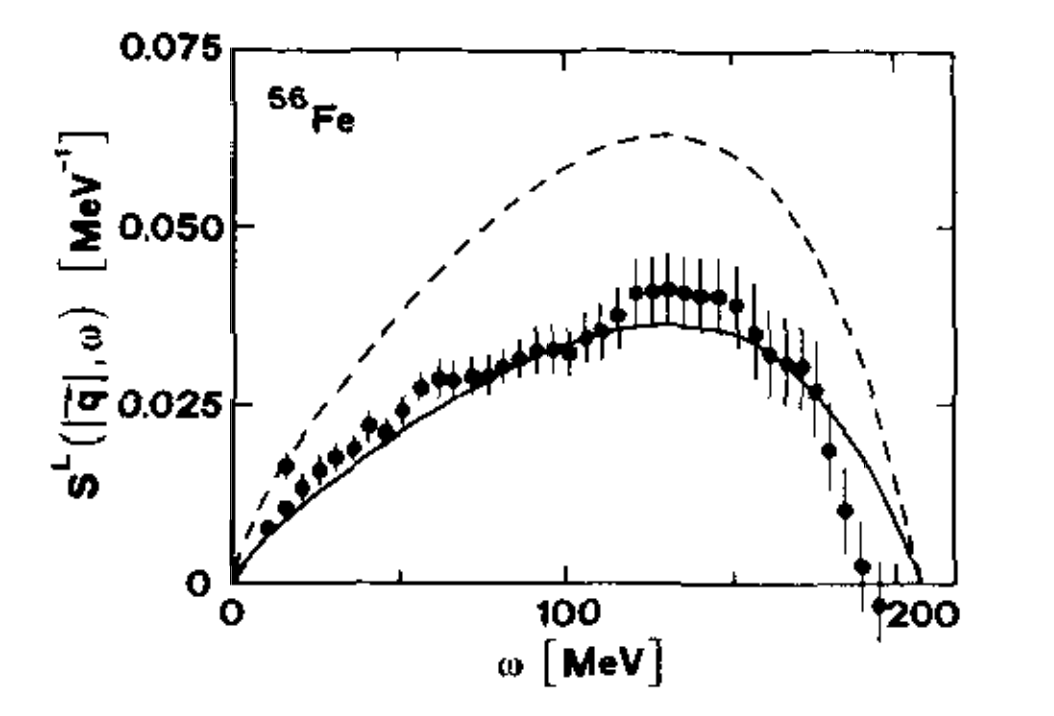
\includegraphics[width=0.7\textwidth]{figs/swollen.png}
\caption[swollen]{
Longitudinal structure function in the relativistic FGM calculation of Noble
\cite{Noble1981} for |q| = 410MeV/c($k_f$ = 1.11 fm$^{−1}$). Experimental data from Altemus \cite{Altemus1980}.
Broken curve: impulse aproximation; Full curve: results with scaled root mean square
radius.
Figure reproduced from \cite{Orlandini1991}.
\label{fig:swollen}}
\end{figure}

%\section{Experiment Kinematics}

\cite{*}

%%%%%%%%%%%%%%%%%%%%%%%%%%%%%%%%%%%%%%%%%%%%%%%%%%%%%%%%%%%%%%%%%%%%%%
% -*-latex-*-
